\section{Analysis 3: Do Frozen Models Benefit from Explicit Geometry?}

\paragraph{Motivation and hypotheses.} Idea 5 supplies explicit geometry (depth, segmentation, pose) for norm reasoning. Before training anything, we measure on frozen models what each kind of input contributes. \textbf{H1}: the answer text alone is not sufficient; visual inputs help, and different combinations of inputs help by different amounts. \textbf{H2}: explicit geometry adds usable information beyond the RGB frames it is derived from.

\paragraph{Data and protocol.} From the released 200-item verified split of EgoNormia \citep{rezaei2025egonormia} we keep one item per source video and take the 60 with the sharpest frames, a choice based on image quality alone. Six frozen models answer each item from four input combinations: the answer options only; the options plus estimated depth maps (Depth Anything V2) without RGB; plus five pre-action RGB frames; and plus frames, depth and instance segmentation (YOLOv8n-seg). As a control they also see the same frames three times. Each answer is a separate call with no shared context and counts only if action and justification are both correct. To see where geometry could matter, we also count how often the correct answers of all 1{,}853 items contain a term from a fixed spatial word list.

\begin{figure}[t]
\centering
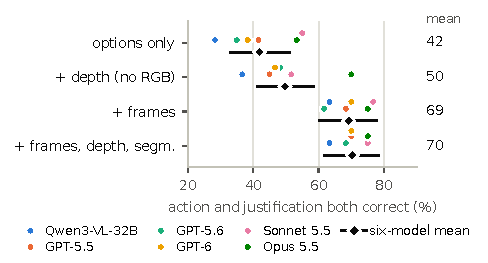
\includegraphics[width=\columnwidth]{analysis3_inputs.pdf}
\caption{Joint accuracy on 60 items for four input combinations. Dots are the six frozen models; the black marker is their mean with a 95\% bootstrap interval over items.}
\label{fig:a3}
\end{figure}

\paragraph{Results.} \emph{H1.} Inputs differ sharply in what they add (Figure~\ref{fig:a3}). Averaged over the six models, the options alone give 42\% (28--55\% by model). A depth map without RGB gives 50\% ($+8$ points, 95\% interval [$-0.3$, 16]; five of six models improve). RGB frames give 69\% ($+27$ points over text [16, 38]; each model $p\le0.03$, exact McNemar), consistent with Analysis~1. \emph{H2.} Adding depth and segmentation to the frames gives 70\%: accuracy changes by $-2$ to $+7$ points per model, $+1.1$ on average [$-1.7$, $+4.2$], with 17 answers corrected and 13 broken across 360 model--item pairs and no model's change significant; the largest is GPT-5.6's gain of four answers ($+7$ points, $p=0.12$). Giving the same frames three times does as well (71\%), and Qwen3-VL-32B scores 39/60 with another item's maps against 38 with its own. Spatial vocabulary is concentrated in Privacy and Proxemics answers (39.5\% and 33.4\%, against 24.6\% overall), yet the 22 Proxemics items score 91 of 132 with or without maps.

\paragraph{Discussion of Analysis 3.} H1 holds and H2 does not. Text alone is not sufficient, and what is added matters: RGB frames add 27 points, a depth map alone about 8, and maps on top of frames nothing. The maps therefore seem informative on their own but redundant beside the frames, even on Proxemics items, where spatial content concentrates. Limits: 60 items detect only large effects (about $\pm12$ points per accuracy), a word list is a coarse measure of spatial content, and sharp verified frames are a best case for the extractors. Most importantly, this does not test Idea 5 itself: these models were presumably never trained to read depth or segmentation maps beside RGB, so a frozen model cannot be expected to use them. Fine-tuning a model on such inputs is the real test, and it is our next experiment.
